\let\negmedspace\undefined
\let\negthickspace\undefined
\documentclass[12pt]{article}
\usepackage{cite}
\usepackage{float}
\usepackage{amsmath,amssymb,amsfonts,amsthm}
\usepackage{algorithmic}
\usepackage{graphicx}
\usepackage{textcomp}
\usepackage{xcolor}
\usepackage{txfonts}
\usepackage{listings}
\usepackage{enumitem}
\usepackage{mathtools}
\usepackage{gensymb}
\usepackage{comment}
\usepackage[breaklinks=true]{hyperref}
\usepackage{tkz-euclide} 
\usepackage{listings}
\usepackage{gvv}                                                             
\usepackage{gvv-book}     
\usepackage{xparse}
\usepackage{color}                                            
\usepackage{array}                                            
\usepackage{longtable}                                       
\usepackage{calc}                                             
\usepackage{multirow}
\usepackage{multicol}
\usepackage{hhline}                                           
\usepackage{ifthen}                                           
\usepackage{lscape}
\usepackage{tabularx}
\usepackage{array}
\usepackage{float}
\usepackage{geometry}
\geometry{left=1in, right=1in, top=1in, bottom=1in}


\begin{document}

\begin{enumerate}[label=\textbf{Q.\arabic*.}, start=1, itemsep=2em]

\section*{Q.1 -- Q.5 carry two marks each.}

\item Which of the following is CORRECT with respect to grammar and usage? Mount Everest is \_\_\_\_\_\_\_\_\_\_.

\noindent \textbf{[GATE EC 2016]}

\begin{multicols}{2}
\begin{enumerate}[label=\Alph*.]
    \item the highest peak in the world
    \item highest peak in the world
    \item one of highest peak in the world
    \item one of the highest peak in the world
\end{enumerate}
\end{multicols}

\item The policeman asked the victim of a theft, “What did you \_\_\_\_\_\_\_\_?”

\noindent \textbf{[GATE EC 2016]}

\begin{multicols}{2}
\begin{enumerate}[label=\Alph*.]
    \item loose
    \item lose
    \item loss
    \item lost
\end{enumerate}
\end{multicols}

\item Despite being warned repeatedly by friends and family about his deteriorating health, his smoking habit remained \_\_\_\_\_\_\_\_.

\noindent \textbf{[GATE EC 2016]}

\begin{multicols}{2}
\begin{enumerate}[label=\Alph*.]
    \item incorrigible
    \item invincible
    \item inevitable
    \item inexorable
\end{enumerate}
\end{multicols}

\item A rewording of something written or spoken is a \_\_\_\_\_\_\_\_.

\noindent \textbf{[GATE EC 2016]}

\begin{multicols}{2}
\begin{enumerate}[label=\Alph*.]
    \item paraphrase
    \item paradox
    \item paradigm
    \item paraffin
\end{enumerate}
\end{multicols}

\item In a 500 m race, the ratio of the speeds of two contestants $A$ and $B$ is 3:4. $A$ has a start of 140 m. Then, $A$ wins by \_\_\_\_\_\_\_\_.

\noindent \textbf{[GATE EC 2016]}

\begin{multicols}{4}
\begin{enumerate}[label=\Alph*.]
    \item 10 m
    \item 20 m
    \item 30 m
    \item 40 m
\end{enumerate}
\end{multicols}

\end{enumerate}

\section*{Q.6 -- Q.10 carry two marks each.}
\begin{enumerate}[label=\textbf{Q.\arabic*.}, start=6, itemsep=2em]

\item A person travelled 80 km in 6 hours. If a part of the journey was travelled at 10 km/h and the remaining at 18 km/h, the distance travelled at 10 km/h was \_\_\_\_\_\_\_\_.

\noindent \textbf{[GATE EC 2016]}

\begin{multicols}{4}
\begin{enumerate}[label=\Alph*.]
    \item 30 km
    \item 40 km
    \item 50 km
    \item 60 km
\end{enumerate}
\end{multicols}

\item A transporter receives the same number of orders each day. The transport cost is \$10 for the first order of the day and \$8 for each subsequent order. If the total cost per day is \$98, the number of orders received each day is \_\_\_\_\_\_\_\_.

\noindent \textbf{[GATE EC 2016]}

\begin{multicols}{4}
\begin{enumerate}[label=\Alph*.]
    \item 11
    \item 12
    \item 13
    \item 14
\end{enumerate}
\end{multicols}

\item A container originally contains 10 litres of pure spirit. From this container, 1 litre of spirit is replaced with 1 litre of water. Subsequently, 1 litre of the mixture is replaced with 1 litre of water and this process is repeated one more time. The ratio of spirit to water in the resulting mixture is \_\_\_\_\_\_\_\_.

\noindent \textbf{[GATE EC 2016]}

\begin{multicols}{4}
\begin{enumerate}[label=\Alph*.]
    \item 729:271
    \item 81:19
    \item 64:27
    \item 343:27
\end{enumerate}
\end{multicols}

\item P, Q, R, S, T, U, V and W are seated around a circular table. R is between V and T; R is opposite P; W is between T and U; P and S are not on either side of U. Who is opposite Q?

\noindent \textbf{[GATE EC 2016]}

\begin{multicols}{4}
\begin{enumerate}[label=\Alph*.]
    \item R
    \item S
    \item T
    \item U
\end{enumerate}
\end{multicols}

\item The data given in the following table summarizes the monthly budget of an average household.

\[
\begin{array}{|c|c|}
\hline
\text{Category} & \text{Expenditure (in \%)} \\
\hline
Food & 35 \\
Housing & 15 \\
Clothing & 10 \\
Transportation & 20 \\
Savings & 10 \\
Other & 10 \\
\hline
\end{array}
\]

Which two categories have identical expenditure?

\noindent \textbf{[GATE EC 2016]}

\begin{multicols}{2}
\begin{enumerate}[label=\Alph*.]
    \item Food and Housing
    \item Housing and Savings
    \item Clothing and Savings
    \item Transportation and Other
\end{enumerate}
\end{multicols}

\section*{Q.1 -- Q.25 carry one mark each.}
\begin{enumerate}[label=\textbf{Q.\arabic*.}]

\item Let $M^4 = I$ (where $I$ denotes the identity matrix) and $M \neq I,\ M^2 \neq I,\ M^3 \neq I$. Then, for any natural number $k$, $M^{-1}$ equals:

\noindent \textbf{[GATE EC 2016]}

\begin{multicols}{2}
\begin{enumerate}[label=\alph*.]
    \item $M^{4k+1}$
    \item $M^{4k+2}$
    \item $M^{4k+3}$
    \item $M^{4k}$
\end{enumerate}
\end{multicols}

\item The second moment of a Poisson-distributed random variable is 2. The mean of the random variable is \rule{2.5cm}{0.4pt}.

\noindent \textbf{[GATE EC 2016]}

\item Given the following statements about a function $f:\mathbb{R}\to\mathbb{R}$, select the right option:

\[
\begin{array}{ll}
\text{P: If }f(x)\text{ is continuous at }x=x_0, \text{ then it is also differentiable at }x=x_0. & \\
\text{Q: If }f(x)\text{ is continuous at }x=x_0, \text{ then it may not be differentiable at }x=x_0. & \\
\text{R: If }f(x)\text{ is differentiable at }x=x_0, \text{ then it is also continuous at }x=x_0. &
\end{array}
\]

\noindent \textbf{[GATE EC 2016]}

\begin{multicols}{2}
\begin{enumerate}[label=\alph*.]
    \item P is true, Q is false, R is false
    \item P is false, Q is true, R is true
    \item P is false, Q is true, R is false
    \item P is true, Q is false, R is true
\end{enumerate}
\end{multicols}

\item Which one of the following is a property of the solutions to the Laplace equation $\nabla^2 f = 0$?

\noindent \textbf{[GATE EC 2016]}

\begin{multicols}{2}
\begin{enumerate}[label=\alph*.]
    \item The solutions have neither maxima nor minima anywhere except at the boundaries.
    \item The solutions are not separable in the coordinates.
    \item The solutions are not continuous.
    \item The solutions are not dependent on the boundary conditions.
\end{enumerate}
\end{multicols}

\item Consider the plot of $f(x)$ versus $x$ as shown below.

\begin{figure}[H]\centering
    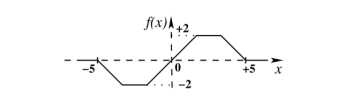
\includegraphics[width=0.6\columnwidth]{figs/q5.png}
    \caption{Plot of $f(x)$.}
    \label{fig:q5}
\end{figure}

Suppose $F(x)=\displaystyle\int_{-5}^{x} f(y)\,dy$. Which one of the following is a graph of $F(x)$?

\noindent \textbf{[GATE EC 2016]}

\begin{figure}[H]\centering
    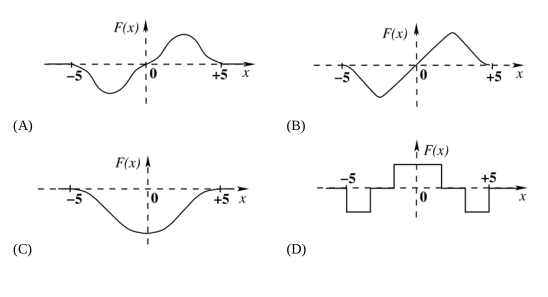
\includegraphics[width=0.6\columnwidth]{figs/q5o.png}
    \caption{options}
    \label{fig:q5o}
\end{figure}

\item Which one of the following is an eigenfunction of the class of all continuous-time, linear, time-invariant systems ( $u(t)$ denotes the unit-step function)?

\noindent \textbf{[GATE EC 2016]}

\begin{multicols}{2}
\begin{enumerate}[label=\alph*.]
    \item $e^{j\omega_0 t} u(t)$
    \item $\cos(\omega_0 t)$
    \item $e^{j\omega_0 t}$
    \item $\sin(\omega_0 t)$
\end{enumerate}
\end{multicols}

\item A continuous-time function $x(t)$ is periodic with period $T$. The function is sampled uniformly with sampling period $T_s$. In which one of the following cases is the sampled signal periodic?

\noindent \textbf{[GATE EC 2016]}

\begin{multicols}{2}
\begin{enumerate}[label=\alph*.]
    \item $T = \sqrt{2}\,T_s$
    \item $T = 1.2\,T_s$
    \item Always
    \item Never
\end{enumerate}
\end{multicols}

\item Consider the sequence $x[n]=a^n u[n]+b^n u[n]$, where $u[n]$ denotes the unit-step sequence and $0<|a|<|b|<1$. The region of convergence (ROC) of the $Z$-transform of $x[n]$ is

\noindent \textbf{[GATE EC 2016]}

\begin{multicols}{2}
\begin{enumerate}[label=\alph*.]
    \item $|z|>|a|$
    \item $|z|>|b|$
    \item $|z|<|a|$
    \item $|a|<|z|<|b|$
\end{enumerate}
\end{multicols}

\item Consider a two-port network with the transmission matrix $T=\myvec{A & B\\ C & D}$. If the network is reciprocal, then

\noindent \textbf{[GATE EC 2016]}

\begin{multicols}{2}
\begin{enumerate}[label=\alph*.]
    \item $T^{-1}=T$
    \item $T^2 = T$
    \item \(\det(T)=0\)
    \item \(\det(T)=1\)
\end{enumerate}
\end{multicols}

\item A continuous-time sinusoid of frequency 33 Hz is multiplied with a periodic Dirac impulse train of frequency 46 Hz. The resulting signal is passed through an ideal analog low-pass filter with cutoff frequency 23 Hz. The fundamental frequency (in Hz) of the output is \rule{2.5cm}{0.4pt}.

\noindent \textbf{[GATE EC 2016]}

\item A small percentage of impurity is added to an intrinsic semiconductor at 300 K. Which one of the following statements is true for the energy band diagram shown in the figure?

\begin{figure}[H]\centering
    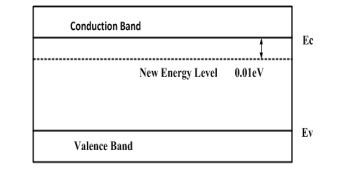
\includegraphics[width=0.55\columnwidth]{figs/q11.png}
    \caption{Energy band diagram (Q.11)}
    \label{fig:q11}
\end{figure}

\noindent \textbf{[GATE EC 2016]}

\begin{multicols}{2}
\begin{enumerate}[label=\alph*.]
    \item Intrinsic semiconductor doped with pentavalent atoms to form n-type semiconductor
    \item Intrinsic semiconductor doped with trivalent atoms to form n-type semiconductor
    \item Intrinsic semiconductor doped with pentavalent atoms to form p-type semiconductor
    \item Intrinsic semiconductor doped with trivalent atoms to form p-type semiconductor
\end{enumerate}
\end{multicols}

\item Consider the following statements for a MOSFET:

\[
\begin{array}{ll}
\text{P: As channel length reduces, OFF-state current increases.} & \\
\text{Q: As channel length reduces, output resistance increases.} & \\
\text{R: As channel length reduces, threshold voltage remains constant.} & \\
\text{S: As channel length reduces, ON current increases.} &
\end{array}
\]

Which of the above statements are INCORRECT?

\noindent \textbf{[GATE EC 2016]}

\begin{multicols}{2}
\begin{enumerate}[label=\alph*.]
    \item P and Q
    \item P and S
    \item Q and R
    \item R and S
\end{enumerate}
\end{multicols}

\item Consider the constant current source shown in the figure. Let $\beta$ represent the current gain of the transistor.

\begin{figure}[H]\centering
    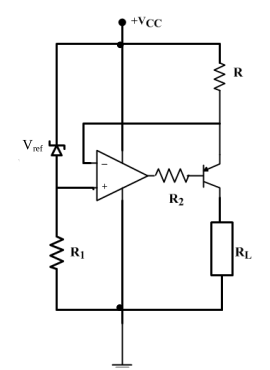
\includegraphics[width=0.55\columnwidth]{figs/q13.png}
    \caption{Constant current source (Q.13)}
    \label{fig:q13}
\end{figure}

The load current $I_0$ through $R_L$ is

\noindent \textbf{[GATE EC 2016]}

\begin{multicols}{2}
\begin{enumerate}[label=\alph*.]
    \item \(I_0 = \dfrac{\beta+1}{\beta}\dfrac{V_{\text{ref}}}{R}\)
    \item \(I_0 = \dfrac{\beta}{\beta+1}\dfrac{V_{\text{ref}}}{R}\)
    \item \(I_0 = \dfrac{\beta+1}{\beta}\dfrac{V_{\text{ref}}}{2R}\)
    \item \(I_0 = \dfrac{\beta}{\beta+1}\dfrac{V_{\text{ref}}}{2R}\)
\end{enumerate}
\end{multicols}

\item The following signal $V_i$ of peak voltage 8 V is applied to the non-inverting terminal of an ideal op-amp. The transistor has $V_{BE}=0.7\,$V, $\beta=100$, $V_{LED}=1.5\,$V, $V_{CC}=10\,$V and $-V_{CC}=-10\,$V.

\begin{figure}[H]\centering
    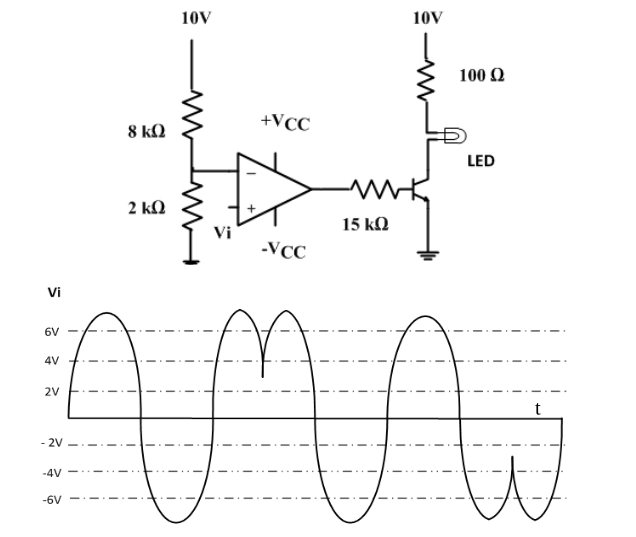
\includegraphics[width=0.65\columnwidth]{figs/q14.png}
    \caption{Signal and LED circuit (Q.14)}
    \label{fig:q14}
\end{figure}

The number of times the LED glows is \rule{2.5cm}{0.4pt}.

\noindent \textbf{[GATE EC 2016]}

\item Consider the oscillator circuit shown in the figure. The function of the network (100 k$\Omega$ in series with two back-to-back diodes) shown in dotted lines is to:

\begin{figure}[H]\centering
    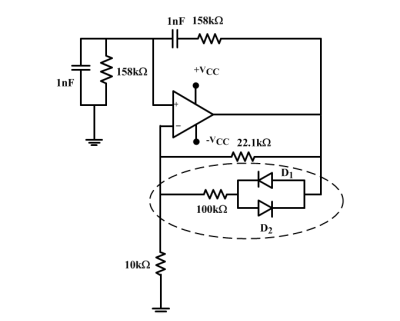
\includegraphics[width=0.6\columnwidth]{figs/q15.png}
    \caption{Oscillator (Q.15)}
    \label{fig:q15}
\end{figure}

\noindent \textbf{[GATE EC 2016]}

\begin{multicols}{2}
\begin{enumerate}[label=\alph*.]
    \item introduce amplitude stabilization by preventing the op amp from saturating and thus producing sinusoidal oscillations of fixed amplitude
    \item introduce amplitude stabilization by forcing the op amp to swing between positive and negative saturation and thus producing square wave oscillations of fixed amplitude
    \item introduce frequency stabilization by forcing the circuit to oscillate at a single frequency
    \item enable the loop gain to take on a value that produces square wave oscillations
\end{enumerate}
\end{multicols}

\item The block diagram of a frequency synthesizer consisting of a Phase Locked Loop (PLL) and a divide-by-\(N\) counter (comprising \(\div 2\), \(\div 4\), \(\div 8\), \(\div 16\) outputs) is sketched below. The synthesizer is excited with a \(5~\mathrm{kHz}\) signal (Input 1). The free-running frequency of the PLL is set to \(20~\mathrm{kHz}\). Assume that the commutator switch makes contacts repeatedly in the order 1-2-3-4.

\begin{figure}[H]\centering
    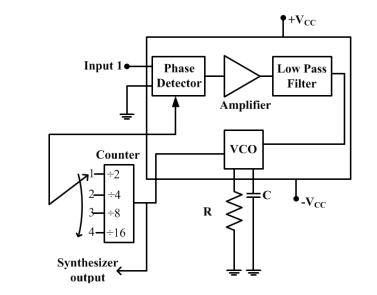
\includegraphics[width=0.6\columnwidth]{figs/q16.png}
    \caption{Combinational circuit (Q.16)}
    \label{fig:q16}
\end{figure}

\noindent \textbf{[GATE EC 2016]}

\begin{multicols}{2}
\begin{enumerate}[label=\alph*.]
    \item 10 kHz, 20 kHz, 40 kHz, 80 kHz
    \item 20 kHz, 40 kHz, 80 kHz, 160 kHz
    \item 80 kHz, 40 kHz, 20 kHz, 10 kHz
    \item 160 kHz, 80 kHz, 40 kHz, 20 kHz
\end{enumerate}
\end{multicols}

\item The output of the combinational circuit given below is:

\begin{figure}[H]\centering
    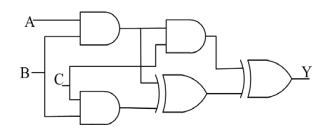
\includegraphics[width=0.6\columnwidth]{figs/q17.png}
    \caption{Combinational circuit (Q.17)}
    \label{fig:q17}
\end{figure}

\noindent \textbf{[GATE EC 2016]}

\begin{multicols}{2}
\begin{enumerate}[label=\alph*.]
    \item $A+B+C$
    \item $A(B+C)$
    \item $B(C+A)$
    \item $C(A+B)$
\end{enumerate}
\end{multicols}

\item What is the voltage $V_{\text{out}}$ in the circuit shown?

\begin{figure}[H]\centering
    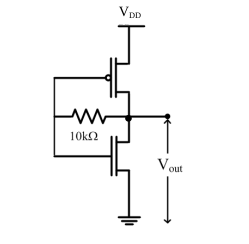
\includegraphics[width=0.6\columnwidth]{figs/q18.png}
    \caption{Circuit for Q.18}
    \label{fig:q18}
\end{figure}

\noindent \textbf{[GATE EC 2016]}

\begin{multicols}{2}
\begin{enumerate}[label=\alph*.]
    \item $0\,$V
    \item $(|V_{T,p}|+V_{T,n})/2$
    \item Switching threshold of inverter
    \item $V_{DD}$
\end{enumerate}
\end{multicols}

\item Match the inferences X, Y, Z about a system to properties P, Q, R of the first column in Routh's table:

\[
\begin{array}{ll}
\text{X: The system is stable …} & \\
\text{Y: The system is unstable …} & \\
\text{Z: The test breaks down …} &
\end{array}
\qquad
\begin{array}{ll}
\text{P: … when all elements are positive} & \\
\text{Q: … when any one element is zero} & \\
\text{R: … when there is a change in sign of coefficients} &
\end{array}
\]

\noindent \textbf{[GATE EC 2016]}

\begin{multicols}{2}
\begin{enumerate}[label=\alph*.]
    \item X→P, Y→Q, Z→R
    \item X→Q, Y→P, Z→R
    \item X→R, Y→Q, Z→P
    \item X→P, Y→R, Z→Q
\end{enumerate}
\end{multicols}

\item A closed-loop control system is stable if the Nyquist plot of the corresponding open-loop transfer function

\noindent \textbf{[GATE EC 2016]}

\begin{multicols}{2}
\begin{enumerate}[label=\alph*.]
    \item encircles the s-plane point $(-1+j0)$ in the counterclockwise direction as many times as the number of right-half s-plane poles.
    \item encircles the s-plane point $(0-j1)$ in the clockwise direction as many times as the number of right-half s-plane poles.
    \item encircles the s-plane point $(-1+j0)$ in the counterclockwise direction as many times as the number of left-half s-plane poles.
    \item encircles the s-plane point $(-1+j0)$ in the counterclockwise direction as many times as the number of right-half s-plane zeros.
\end{enumerate}
\end{multicols}

\item Consider binary data transmission at a rate of 56 kbps using baseband binary PAM designed to have a raised-cosine spectrum. The transmission bandwidth (in kHz) required for a roll-off factor of 0.25 is \rule{2.5cm}{0.4pt}.

\noindent \textbf{[GATE EC 2016]}

\item A superheterodyne receiver operates in the frequency range 58 MHz–68 MHz. The intermediate frequency $f_{\text{IF}}$ and local oscillator frequency $f_{\text{LO}}$ are chosen such that $f_{\text{IF}}\le f_{\text{LO}}$. It is required that the image frequencies fall outside the 58–68 MHz band. The minimum required $f_{\text{IF}}$ (in MHz) is \rule{2.5cm}{0.4pt}.

\noindent \textbf{[GATE EC 2016]}

\item The amplitude of a sinusoidal carrier is modulated by a single sinusoid to obtain the AM signal
\[
s(t)=5\cos(1600\pi t)+20\cos(1800\pi t)+5\cos(2000\pi t).
\]
The modulation index is \rule{2.5cm}{0.4pt}.

\noindent \textbf{[GATE EC 2016]}

\item Concentric spherical shells of radii 2 m, 4 m and 8 m carry uniform surface charge densities of $20\,$nC/m$^2$, $-4\,$nC/m$^2$ and $\rho_s$, respectively. The value of $\rho_s$ (nC/m$^2$) required to ensure that the electric flux density $\mathbf{D}=\mathbf{0}$ at radius 10 m is \rule{2.5cm}{0.4pt}.

\noindent \textbf{[GATE EC 2016]}

\item The propagation constant of a lossy transmission line is $(2+j5)\,\text{m}^{-1}$ and its characteristic impedance is $(50+j0)\,\Omega$ at $\omega=10^6\,\text{rad/s}$. The values of the line constants $L,C,R,G$ are, respectively:

\noindent \textbf{[GATE EC 2016]}

\begin{multicols}{2}
\begin{enumerate}[label=\alph*.]
    \item $L=200\ \mu\mathrm{H/m},\ C=0.1\ \mu\mathrm{F/m},\ R=50\ \Omega/\mathrm{m},\ G=0.02\ \mathrm{S/m}$
    \item $L=250\ \mu\mathrm{H/m},\ C=0.1\ \mu\mathrm{F/m},\ R=100\ \Omega/\mathrm{m},\ G=0.04\ \mathrm{S/m}$
    \item $L=200\ \mu\mathrm{H/m},\ C=0.2\ \mu\mathrm{F/m},\ R=100\ \Omega/\mathrm{m},\ G=0.02\ \mathrm{S/m}$
    \item $L=250\ \mu\mathrm{H/m},\ C=0.2\ \mu\mathrm{F/m},\ R=50\ \Omega/\mathrm{m},\ G=0.04\ \mathrm{S/m}$
\end{enumerate}
\end{multicols}

\end{enumerate}

\newpage
\section*{Q.26 -- Q.55 carry two marks each.}
\begin{enumerate}[label=\textbf{Q.\arabic*.}, start=26]

\item Evaluate
\[
\frac{1}{2\pi}\iint_{D} (x+y+10)\,dx\,dy,
\]
where \(D\) denotes the disc \(x^2+y^2\le 4\). The value is \rule{3cm}{0.4pt}.

\noindent \textbf{[GATE EC 2016]}

\item A sequence $x[n]$ is specified as
\[
\begin{pmatrix} x[n] \\ x[n-1] \end{pmatrix}
=
\begin{pmatrix} 1 & 1 \\[3pt] 1 & 0 \end{pmatrix}^n
\begin{pmatrix} 1 \\[3pt] 0 \end{pmatrix}, \quad \text{for } n\ge 2.
\]
The initial conditions are $x[0]=1$, $x[1]=1$, and $x[n]=0$ for $n<0$. The value of $x[12]$ is \rule{3cm}{0.4pt}.

\noindent \textbf{[GATE EC 2016]}

\item In the integral below the contour $C$ encloses the points $2\pi j$ and $-2\pi j$:
\[
\frac{1}{2\pi j}\oint_{C}\frac{\sin z}{(z-2\pi j)^3}\,dz.
\]
The value of the integral is \rule{3cm}{0.4pt}.

\noindent \textbf{[GATE EC 2016]}

\item The region specified by \(\{(\rho,\phi,z): 3\le \rho\le 5,\ \tfrac{\pi}{8}\le\phi\le\tfrac{\pi}{4},\ 3\le z\le 4.5\}\) in cylindrical coordinates has volume of \rule{3cm}{0.4pt}.

\noindent \textbf{[GATE EC 2016]}

\item The Laplace transform of the causal periodic square wave of period $T$ shown in the figure below is:

\begin{figure}[H]\centering
    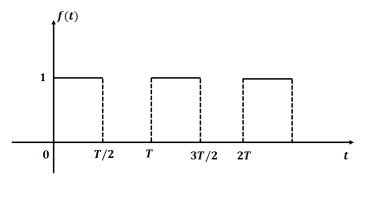
\includegraphics[width=0.6\columnwidth]{figs/q30.png}
    \caption{Periodic square wave (Q.30)}
    \label{fig:q30}
\end{figure}

\noindent \textbf{[GATE EC 2016]}

\begin{multicols}{2}
\begin{enumerate}[label=\alph*.]
    \item \(F(s)=\dfrac{1}{1+e^{-sT/2}}\)
    \item \(F(s)=\dfrac{1}{s\big(1+e^{-sT/2}\big)}\)
    \item \(F(s)=\dfrac{1}{s(1-e^{-sT})}\)
    \item \(F(s)=\dfrac{1}{1-e^{-sT}}\)
\end{enumerate}
\end{multicols}

\begin{enumerate}[label=\textbf{Q.\arabic*.}, start=31]

\item A network consisting of a finite number of linear resistor (R), inductor (L), and capacitor (C)
elements, connected all in series or all in parallel, is excited with a source of the form
\[
\sum_{k=1}^{3} a_k\cos(k\omega_0 t),\quad\text{where } a_k\neq 0,\ \omega_0\neq 0.
\]
The source has nonzero impedance. Which one of the following is a possible form of the output
measured across a resistor in the network?

\noindent \textbf{[GATE EC 2016]}

\begin{multicols}{2}
\begin{enumerate}[label=\alph*.]
    \item $\displaystyle \sum_{k=1}^{3} b_k\cos(k\omega_0 t + \phi_k),\ \text{where } b_k \neq a_k\ \forall k$
    \item $\displaystyle \sum_{k=1}^{4} b_k\cos(k\omega_0 t + \phi_k),\ \text{where } b_k \neq 0\ \forall k$
    \item $\displaystyle \sum_{k=1}^{3} a_k\cos(k\omega_0 t + \phi_k)$
    \item $\displaystyle \sum_{k=1}^{2} a_k\cos(k\omega_0 t + \phi_k)$
\end{enumerate}
\end{multicols}

\item A first-order low-pass filter of time constant $T$ is excited with different input signals (with zero initial conditions up to $t=0$). Match the excitation signals X, Y, Z with the corresponding time responses for $t\ge0$:

\[
\begin{array}{ll}
\text{X: Impulse} & \text{P: }1-e^{-t/T} \\
\text{Y: Unit step} & \text{Q: }t - T\big(1-e^{-t/T}\big) \\
\text{Z: Ramp} & \text{R: }e^{-t/T}
\end{array}
\]

\noindent \textbf{[GATE EC 2016]}

\begin{multicols}{2}
\begin{enumerate}[label=\alph*.]
    \item X → R,\; Y → Q,\; Z → P
    \item X → Q,\; Y → P,\; Z → R
    \item X → R,\; Y → P,\; Z → Q
    \item X → P,\; Y → R,\; Z → Q
\end{enumerate}
\end{multicols}

\item An AC voltage source $V=10\sin(t)$ volts is applied to the network shown in the figure. Assume $R_1=3\ \text{k}\Omega$, $R_2=6\ \text{k}\Omega$ and $R_3=9\ \text{k}\Omega$, and that the diode is ideal.

\begin{figure}[H]\centering
    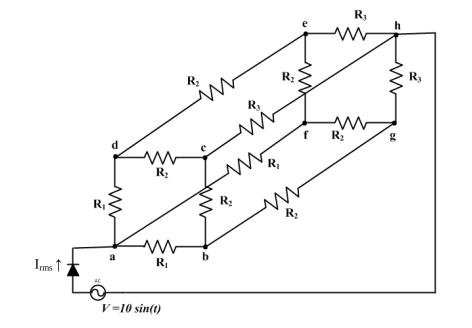
\includegraphics[width=0.6\columnwidth]{figs/q33.png}
    \caption{Network for Q.33}
    \label{fig:q33}
\end{figure}

RMS current $I_{\text{rms}}$ (in mA) through the diode is \rule{3cm}{0.4pt}.

\noindent \textbf{[GATE EC 2016]}

\item In the circuit shown, the maximum power (in watt) delivered to the resistor $R$ is \rule{3cm}{0.4pt}.

\begin{figure}[H]\centering
    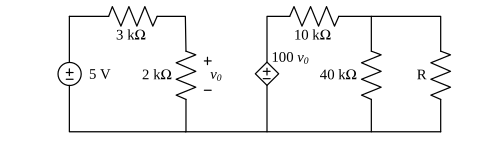
\includegraphics[width=0.6\columnwidth]{figs/q34.png}
    \caption{Circuit for Q.34}
    \label{fig:q34}
\end{figure}

\noindent \textbf{[GATE EC 2016]}

\item Consider the signal
\[
x[n]=6\delta[n+2]+3\delta[n+1]+8\delta[n]+7\delta[n-1]+4\delta[n-2].
\]
If $X(e^{j\omega})$ is the discrete-time Fourier transform of $x[n]$, then
\[
\frac{1}{\pi}\int_{-\pi}^{\pi} X(e^{j\omega})\,\sin^2(2\omega)\,d\omega
\]
is equal to \rule{3cm}{0.4pt}.

\noindent \textbf{[GATE EC 2016]}

\item Consider a silicon p–n junction with a uniform acceptor doping concentration of $10^{17}\,\text{cm}^{-3}$ on the p-side and a uniform donor doping concentration of $10^{16}\,\text{cm}^{-3}$ on the n-side. No external voltage is applied to the diode. Given: $kT/q=26\ \text{mV}$, $n_i=1.5\times10^{10}\,\text{cm}^{-3}$, $\varepsilon_{\text{Si}}=12\varepsilon_0$, $\varepsilon_0=8.85\times10^{-14}\,\text{F/m}$, and $q=1.6\times10^{-19}\,$C. The charge per unit junction area (nC cm$^{-2}$) in the depletion region on the p-side is \rule{3cm}{0.4pt}.

\noindent \textbf{[GATE EC 2016]}

\item Consider an n-channel MOSFET with gate-to-source voltage $V_{GS}=1.8\,$V. Assume $W/L=4$, $\mu_n C_{\text{ox}} = 70\times10^{-6}\,\text{A/V}^2$, threshold voltage $V_T=0.3\,$V, and channel-length modulation parameter $\lambda=0.09\ \text{V}^{-1}$. In the saturation region, the drain conductance (in µS) is \rule{3cm}{0.4pt}.

\noindent \textbf{[GATE EC 2016]}

\item The figure below shows the doping distribution in a p-type semiconductor (log scale). The magnitude of the electric field (in kV/cm) in the semiconductor due to non-uniform doping is \rule{3cm}{0.4pt}.

\begin{figure}[H]\centering
    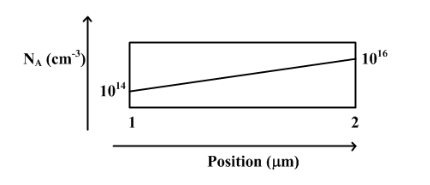
\includegraphics[width=0.6\columnwidth]{figs/q38.png}
    \caption{Doping profile (Q.38)}
    \label{fig:q38}
\end{figure}

\noindent \textbf{[GATE EC 2016]}

\item Consider a silicon sample at $T = 300\,$K, with uniform donor density $N_d = 5\times 10^{16}\ \text{cm}^{-3}$, illuminated uniformly with an optical generation rate of $G_{\text{opt}} = 1.5\times 10^{20}\ \text{cm}^{-3}\text{s}^{-1}$. The incident radiation is turned off at $t=0$. Assume low-level injection and ignore surface effects. The carrier lifetimes are $\tau_{p0} = 0.1\,\mu\text{s}$ and $\tau_{n0} = 0.5\,\mu\text{s}$. The excess carrier concentrations $\Delta n$ and $\Delta p$ immediately after $t=0$ are

\noindent \textbf{[GATE EC 2016]}

\begin{figure}[H]\centering
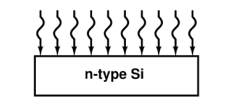
\includegraphics[width=0.55\columnwidth]{figs/q39.png}
\caption{Silicon sample under optical illumination}
\label{fig:q39}
\end{figure}

\begin{multicols}{2}
    \begin{enumerate}
        \item $1.5\times 10^{13}\ \text{cm}^{-3}$ and $7.47\times 10^{11}\ \text{cm}^{-3}$
        \item $1.5\times 10^{13}\ \text{cm}^{-3}$ and $8.23\times 10^{11}\ \text{cm}^{-3}$
        \item $7.5\times 10^{13}\ \text{cm}^{-3}$ and $3.73\times 10^{11}\ \text{cm}^{-3}$
        \item $7.5\times 10^{13}\ \text{cm}^{-3}$ and $4.12\times 10^{11}\ \text{cm}^{-3}$
    \end{enumerate}
\end{multicols}

\item An ideal op-amp has voltage sources $V_1, V_3, V_5,\dots, V_{N-1}$ connected to the non-inverting input and $V_2, V_4, V_6,\dots, V_N$ connected to the inverting input as shown. The voltages are $1, -\tfrac{1}{2}, \tfrac{1}{3}, -\tfrac{1}{4}, \dots$ volts, respectively. As $N \to \infty$, the output voltage (in volt) is \_\_\_\_\_\_\_.

\noindent \textbf{[GATE EC 2016]}

\begin{figure}[H]\centering
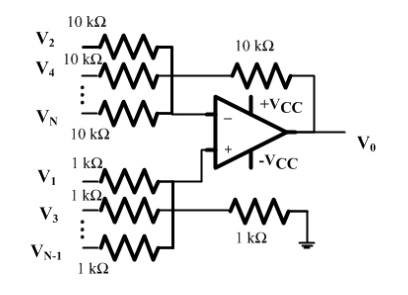
\includegraphics[width=0.6\columnwidth]{figs/q40.png}
\caption{Op-amp with infinite input series}
\label{fig:q40}
\end{figure}

\item A p-i-n photodiode of responsivity $0.8\ \text{A/W}$ is connected to the inverting input of an ideal op-amp as shown. If $10\ \mu$W optical power is incident, the photocurrent (in $\mu$A) through the load resistor $R_L = 10\,$k$\Omega$ is \_\_\_\_\_\_\_.

\noindent \textbf{[GATE EC 2016]}

\begin{figure}[H]\centering
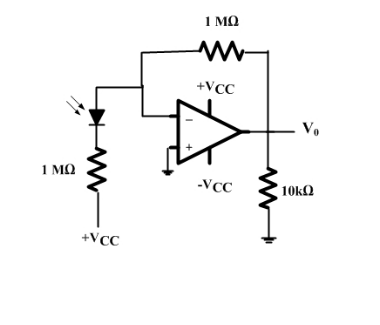
\includegraphics[width=0.55\columnwidth]{figs/q41.png}
\caption{Photodiode with op-amp load}
\label{fig:q41}
\end{figure}

\item Identify the circuit below.

\noindent \textbf{[GATE EC 2016]}

\begin{figure}[H]\centering
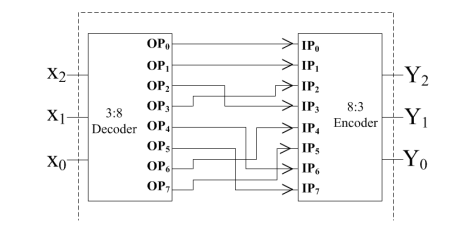
\includegraphics[width=0.5\columnwidth]{figs/q42.png}
\caption{Logic circuit}
\label{fig:q42}
\end{figure}

\begin{multicols}{2}
    \begin{enumerate}
        \item Binary to Gray code converter
        \item Binary to XS-3 converter
        \item Gray to Binary converter
        \item XS-3 to Binary converter
    \end{enumerate}
\end{multicols}

\item The functionality implemented by the circuit shown is

\noindent \textbf{[GATE EC 2016]}

\begin{figure}[H]\centering
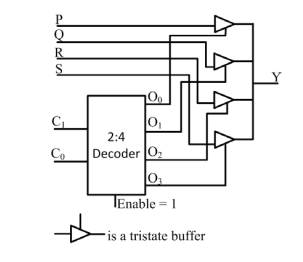
\includegraphics[width=0.55\columnwidth]{figs/q43.png}
\caption{Combinational logic circuit}
\label{fig:q43}
\end{figure}

\begin{multicols}{2}
    \begin{enumerate}
        \item 2-to-1 multiplexer
        \item 4-to-1 multiplexer
        \item 7-to-1 multiplexer
        \item 6-to-1 multiplexer
    \end{enumerate}
\end{multicols}

\item In an 8085 system, a PUSH requires more cycles than a POP. The reason is

\noindent \textbf{[GATE EC 2016]}

\begin{multicols}{2}
    \begin{enumerate}
        \item POP uses memory→processor like fetch, PUSH reverses direction
        \item Memory write is slower than memory read
        \item Stack pointer must pre-decrement before PUSH
        \item Order of registers is interchanged for PUSH
    \end{enumerate}
\end{multicols}

\item The open-loop transfer function of a unity-feedback system is
\[
G(s) = \frac{K}{s^2 + 5s + 5}.
\]

\noindent \textbf{[GATE EC 2016]}

The value of $K$ at the breakaway point of the root-locus is \_\_\_\_\_\_\_.

\item For
\[
G(s) = \frac{K}{s(s+2)},
\]

\noindent \textbf{[GATE EC 2016]}

the value of $K$ for $10\%$ peak overshoot is \_\_\_\_\_\_\_.

\item The transfer function
\[
H(s) = 2s^{4} - 5s^{3} + 5s - 2
\]

\noindent \textbf{[GATE EC 2016]}

has how many zeros in the right half-plane? \_\_\_\_\_\_\_

\item A discrete memoryless source with alphabet $S = \{s_0, s_1, \dots\}$ and probabilities
\[
P = \left\{\tfrac{1}{2}, \tfrac{1}{4}, \tfrac{1}{8}, \tfrac{1}{16}, \dots \right\}
\]

\noindent \textbf{[GATE EC 2016]}

has entropy (bits) equal to \_\_\_\_\_\_\_.

\item A 3-repetition code is used over a BSC with $p=0.1$, with majority decoding. The average probability of error is \_\_\_\_\_\_\_.

\noindent \textbf{[GATE EC 2016]}

\item An analog pulse $s(t)$ is transmitted over AWGN. At filter output, $\mathrm{SNR}_{\max}$ equals?

\noindent \textbf{[GATE EC 2016]}

\begin{multicols}{2}
    \begin{enumerate}
        \item $E_s = E_h$, $\ \mathrm{SNR}_{\max} = 2E_s/N_0$
        \item $E_s = E_h$, $\ \mathrm{SNR}_{\max} = E_s/2N_0$
        \item $E_s > E_h$, $\ \mathrm{SNR}_{\max} > 2E_s/N_0$
        \item $E_s < E_h$, $\ \mathrm{SNR}_{\max} = 2E_h/N_0$
    \end{enumerate}
\end{multicols}

\item Current density
\[
\mathbf{J} = \frac{400\sin\theta}{2\pi(r^{2}+4)}\hat{a}_r \ \text{A/m}^2
\]

\noindent \textbf{[GATE EC 2016]}

The total current and average current density through surface $r=0.8\,$m, $\pi/12 \le \theta \le \pi/4$ are

\begin{multicols}{2}
    \begin{enumerate}
        \item $15.09$ A,\ $12.86$ A/m$^2$
        \item $18.73$ A,\ $13.65$ A/m$^2$
        \item $12.86$ A,\ $9.23$ A/m$^2$
        \item $10.28$ A,\ $7.56$ A/m$^2$
    \end{enumerate}
\end{multicols}

\item Antenna with $T_{ant}=50$K, amplifier NF $=2$ dB, BW $=12$ MHz. Find $T_e$ and $P_{ao}$.

\noindent \textbf{[GATE EC 2016]}

\begin{multicols}{2}
    \begin{enumerate}
        \item $T_e=169.36$ K,\ $P_{ao}=3.73\times10^{-10}$ W
        \item $T_e=170.8$ K,\ $P_{ao}=4.56\times10^{-10}$ W
        \item $T_e=182.5$ K,\ $P_{ao}=3.85\times10^{-10}$ W
        \item $T_e=160.62$ K,\ $P_{ao}=4.6\times10^{-10}$ W
    \end{enumerate}
\end{multicols}

\item Two horn antennas, distance $200\lambda$, $\Gamma_t=0.15$, $\Gamma_r=0.18$, $G_t=18$ dB, $G_r=22$ dB, $P_{in}=2$ W. Power delivered at receiver (mW) is \_\_\_\_\_\_\_.

\noindent \textbf{[GATE EC 2016]}

\item Incident field
\[
\mathbf{E}_{\text{inc}} = (\hat{a}_x + j\hat{a}_y)E_0 e^{jkz}, \qquad
\mathbf{E}_a = (\hat{a}_x + 2\hat{a}_y)\frac{E_I}{r}e^{-jkr}
\]

\noindent \textbf{[GATE EC 2016]}

Polarization and mismatch loss are

\begin{multicols}{2}
    \begin{enumerate}
        \item Linear,\ Circular (CW), $-5$ dB
        \item Circular (CW), Linear,\ $-5$ dB
        \item Circular (CW), Linear,\ $-3$ dB
        \item Circular (ACW), Linear,\ $-3$ dB
    \end{enumerate}
\end{multicols}

\item Helical antenna with far-zone density
\[
W_{\text{rad}}(\hat{r}) = \frac{a r C_0}{r^2}\cos^{4}\theta
\]

\noindent \textbf{[GATE EC 2016]}

Radiated power and directivity are

\begin{multicols}{2}
    \begin{enumerate}
        \item $1.5C_0$, 10 dB
        \item $1.256C_0$, 10 dB
        \item $1.256C_0$, 12 dB
        \item $1.5C_0$, 12 dB
    \end{enumerate}
\end{multicols}

\end{enumerate}

\end{enumerate}

\end{enumerate}

\end{document}
